% Rewrite example (financial, Haiku): from out/rewrite; lost requirements marked. Clause version answered right.
% Shared setup for the diagrams (teaser, pipeline, worked). Built with XeLaTeX so that all text is Arial, in black.
% Sizes match the paper's acmart sigconf sizes (\footnotesize 7 pt); the smallest text is 6 pt.
\documentclass[border=0.5pt]{standalone}
\usepackage{fontspec}
\setmainfont{Arial}\setsansfont{Arial}\setmonofont{Menlo}[Scale=MatchLowercase]
\usepackage{unicode-math}\setmathfont{FiraMath-Regular.otf}
\usepackage{booktabs}
\usepackage{tikz}
\usetikzlibrary{arrows.meta,calc,positioning,fit,backgrounds,shapes.geometric}
\renewcommand\large{\fontsize{10}{12}\selectfont}
\renewcommand\small{\fontsize{8}{10}\selectfont}
\renewcommand\footnotesize{\fontsize{7}{8.4}\selectfont}
\renewcommand\scriptsize{\fontsize{6.5}{7.6}\selectfont}
\renewcommand\tiny{\fontsize{6}{7}\selectfont}
\newcommand{\nohyph}{\hyphenpenalty=10000\exhyphenpenalty=10000\relax}
\newcommand{\sql}[1]{\texttt{#1}}
% the edited SQL clause, highlighted as in AMBROSIA and the test-suite paper; plain check and cross marks
\newcommand{\hl}[2]{{\setlength{\fboxsep}{0.7pt}\colorbox{#1f}{\vphantom{Ay}\texttt{#2}}}}
\newfontfamily\markfont{Arial Unicode MS}\newcommand{\yes}{{\markfont ✓}}\newcommand{\no}{{\markfont ✗}}
% math letters in Arial italic; the open-request circle is drawn; only the arrow comes from Fira Math
\newcommand{\vq}[1]{\textit{q}\textsubscript{#1}}\newcommand{\vp}[1]{\textit{p}\textsubscript{#1}}\newcommand{\vo}{\mbox{\textit{q}\hspace{0.3pt}\raisebox{-0.25ex}{\tikz[baseline=0pt]\draw[line width=0.45pt] (0,1.1pt) circle (1.1pt);}}}
% box lines: A (blue) and B (orange) as in the data figures; neutral lines grey. Text is always black.
% colors as in AMBROSIA's and AmbiQT's diagrams (draw.io palette): interpretation A blue, interpretation B orange, code blocks light gray
\definecolor{sbA}{HTML}{6C8EBF}\definecolor{sbB}{HTML}{D79B00}\definecolor{sbAf}{HTML}{DAE8FC}\definecolor{sbBf}{HTML}{FFE6CC}\definecolor{sbline}{HTML}{4D4D4D}
\definecolor{sbfill}{HTML}{F5F5F5}

\definecolor{lostf}{HTML}{F8CECC}
\begin{document}
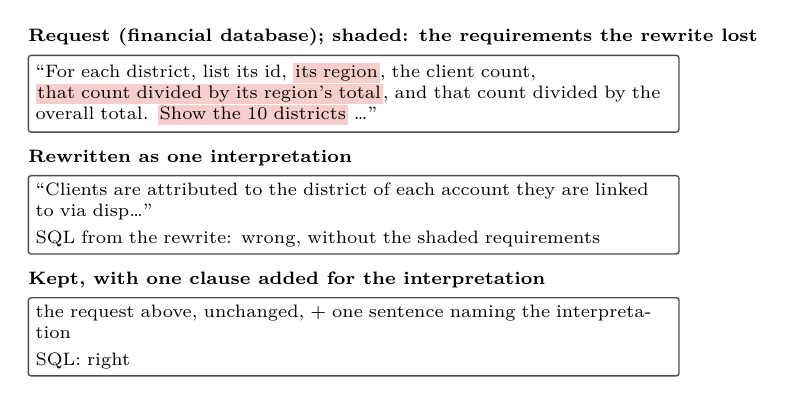
\begin{tikzpicture}[x=1cm, y=1cm, font=\scriptsize, >=Stealth, line width=0.5pt,
  bx/.style={draw=sbline, rounded corners=1pt, inner sep=2.6pt, align=left, text width=8.08cm, anchor=north west},
  st/.style={font=\scriptsize\bfseries, anchor=north west, inner sep=0pt}]
\newcommand{\lost}[1]{{\setlength{\fboxsep}{0.7pt}\colorbox{lostf}{\vphantom{Ay}#1}}}
\node[st] (h1) at (0,0) {Request (financial database); shaded: the requirements the rewrite lost};
\node[bx] (q) at ([yshift=-3pt]h1.south west) {``For each district, list its id, \lost{its region}, the client count, \lost{that count divided by its region's total}, and that count divided by the overall total. \lost{Show the 10 districts} \ldots''};
\node[st] (h2) at ([yshift=-6pt]q.south west) {Rewritten as one interpretation};
\node[bx] (r) at ([yshift=-3pt]h2.south west) {``Clients are attributed to the district of each account they are linked to via disp\ldots''\\[2pt]
SQL from the rewrite: wrong, without the shaded requirements};
\node[st] (h3) at ([yshift=-6pt]r.south west) {Kept, with one clause added for the interpretation};
\node[bx] (c) at ([yshift=-3pt]h3.south west) {the request above, unchanged, + one sentence naming the interpretation\\[2pt] SQL: right};
\end{tikzpicture}
\end{document}
